\documentclass[a4paper, 11pt]{article}

% Packages
\usepackage[utf8]{inputenc}
\usepackage[T1]{fontenc}
\usepackage[english]{babel}
\usepackage{amsmath, amssymb, amsthm}
\usepackage{geometry}
\usepackage{graphicx}
\usepackage{hyperref}
\usepackage{algorithm}
\usepackage{algpseudocode}
\usepackage{booktabs}
\usepackage{microtype}
\usepackage{tikz}
\usetikzlibrary{matrix,positioning,arrows.meta,calc}

% Layout
\geometry{left=2.5cm, right=2.5cm, top=3cm, bottom=3cm}

% Theorems
\newtheorem{theorem}{Theorem}
\newtheorem{definition}{Definition}
\newtheorem{lemma}{Lemma}
\newtheorem{corollary}{Corollary}

% Metadata
\title{\textbf{Directed Synergy: Solving the Plasticity-Stability Dilemma via Contextual Gating}}
\author{Dipl.-Inf. Sven Jansen}
\date{December 2024}

\begin{document}

\maketitle

\begin{abstract}
Continual learning in neural networks aims to resolve the \textbf{Plasticity-Stability Dilemma}: how to learn new tasks (plasticity) without erasing old knowledge (stability). While strict architectural separation offers a theoretical guarantee against forgetting, our experiments show that in deep transformers with shared embeddings, "Strict Separation" is often intractable due to leakage ("Leakage Creep"). We introduce \textbf{Directed Synergy with Contextual Gating}, a pragmatic framework that combines architectural gating with \textbf{Asymmetric Experience Replay}. By employing \textbf{Bigram Routers} to disambiguate task contexts and \textbf{Zero Initialization} to enable soft separation, DGE achieves high plasticity (Loss $\approx 1.0$) and perfect stability (Probe Loss $\approx 2.0$), solving the dilemma where static isolation failed.
\end{abstract}

\section{Introduction: The Pragmatics of Continual Learning}

The Plasticity-Stability Dilemma remains the central challenge of continual learning. Approaches typically fall into three categories: Regularization (EWC), Replay (ER), and Architecture (MoE/Adapters).

\subsection{The Failure of Strict Separation}
Our investigation revealed that relying solely on architectural barriers ("Strict Separation") is fragile in deep networks:
\begin{itemize}
    \item \textbf{MLP Routers}: Suffer from OOD generalization. Even with hard thresholding, small activations leak and amplify through layers ("Leakage Creep"), leading to catastrophic forgetting.
    \item \textbf{RBF Routers}: While geometrically sound for separation, they scale poorly (Cost $O(N^2)$ or OOM) and suffer from "Dead Gates" in high dimensions.
\end{itemize}

\subsection{The DGE Proposal: Directed Synergy}
Instead of chasing perfect isolation, we propose \textbf{Directed Synergy}: using DGE gates to \emph{bias} the network towards separation, while using \textbf{Asymmetric Replay} to provide the necessary gradients to maintain stability. The key innovations are:
\begin{enumerate}
    \item \textbf{Dual-Gate Architecture}: Separate Forward ($G_{fwd}$) and Backward ($G_{bwd}$) gates to decouple inference capacity from training updates.
    \item \textbf{Contextual Gating}: Using \textbf{Bigram Routers} to allow the network to distinguish tasks based on transition context ($t-1 \to t$).
    \item \textbf{Asymmetric Replay}: Freezing new weights during replay to force the router to learn strict separation.
\end{enumerate}

\section{The Dual-Gate Architecture}

\subsection{Core Principle: Separate Control Channels}

For a weight matrix $W \in \mathbb{R}^{n \times k}$, we introduce two independent gate systems:

\begin{equation}
    \text{Forward Gate: } G_{fwd} = \sigma(g^{row}_{fwd} \oplus g^{col}_{fwd})
\end{equation}

\begin{equation}
    \text{Backward Gate: } G_{bwd} \in \{0, 1\}^{n \times k}
\end{equation}

Where $\oplus$ denotes the outer sum ($g^{row}_i + g^{col}_j$) and $\sigma$ is the sigmoid function.

\subsection{Forward Pass}

During inference, the effective weight matrix is:
\begin{equation}
    W_{eff} = W \odot G_{fwd}
\end{equation}

The output is computed as:
\begin{equation}
    y = W_{eff} \cdot x = (W \odot G_{fwd}) \cdot x
\end{equation}

\subsection{Backward Pass (Soft Separation)}

During training, we intercept the gradient update:
\begin{equation}
    \nabla W := \nabla W \odot G_{bwd} + \text{Rescue}
\end{equation}

Unlike strict masking, we acknowledge that gradients permeate through shared embeddings. Therefore, we ensure stability through:

\subsubsection{Mechanism 1: Zero Initialization}
We initialize new weights $W_{new} \sim \mathcal{N}(0, 0)$ (or very small noise). This ensures that initially, $W_{new} \cdot x \approx 0$.
\begin{enumerate}
    \item \textbf{Replay Stability:} Since $W_{new}$ contributes nothing, it does not disrupt old tasks in the replay buffer.
    \item \textbf{Plasticity Start:} The router $G$ is free to open based on input patterns without incurring immediate high loss penalties.
\end{enumerate}

\subsubsection{Mechanism 2: Gradient Rescue}
To prevent "Dead Gates" (where gates close permanently due to initial instability), we introduce a rescue hook:
\begin{equation}
    \text{If } \mu(G_{fwd}) < \epsilon: \quad \nabla G \gets \nabla G \times \alpha_{boost}
\end{equation}
This forces the router to explore opening gates even if initial gradients suggest closure, maintaining plasticity.

\subsection{The Key Innovation: Decoupling}

The fundamental innovation is that $G_{fwd}$ and $G_{bwd}$ are \textbf{independent}:

\begin{center}
\begin{tabular}{|c|c|l|}
\hline
$G_{fwd}$ & $G_{bwd}$ & Behavior \\
\hline
Open (1) & Open (1) & Normal: Weight is used and trainable \\
Open (1) & Closed (0) & \textbf{Protected}: Weight is used but frozen \\
Closed (0) & Open (1) & Silent: Weight contributes nothing (yet trainable) \\
Closed (0) & Closed (0) & Dormant: Weight is invisible and frozen \\
\hline
\end{tabular}
\end{center}

The ``Protected'' state is the key enabler of continual learning: old knowledge remains accessible ($G_{fwd} = 1$) but immutable ($G_{bwd} = 0$).

\section{Matrix Expansion Topology}

\subsection{Quadrant Structure}

When expanding a matrix from $\mathbb{R}^{n \times k}$ to $\mathbb{R}^{(n+\Delta n) \times (k+\Delta k)}$, we obtain four functional quadrants:

\begin{figure}[h]
\centering
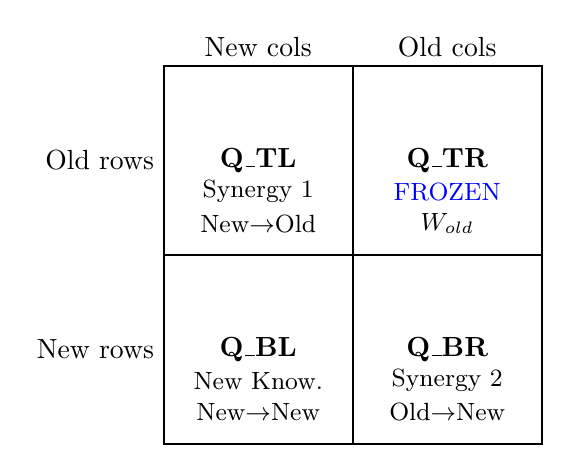
\begin{tikzpicture}[scale=0.8]
    % Draw the matrix
    \draw[thick] (0,0) rectangle (6,6);
    \draw[thick] (3,0) -- (3,6);
    \draw[thick] (0,3) -- (6,3);
    
    % Labels
    \node at (1.5,4.5) {\textbf{Q\_TL}};
    \node at (1.5,4.0) {\small Synergy 1};
    \node at (1.5,3.5) {\small New$\to$Old};
    
    \node at (4.5,4.5) {\textbf{Q\_TR}};
    \node at (4.5,4.0) {\small \textcolor{blue}{FROZEN}};
    \node at (4.5,3.5) {\small $W_{old}$};
    
    \node at (1.5,1.5) {\textbf{Q\_BL}};
    \node at (1.5,1.0) {\small New Know.};
    \node at (1.5,0.5) {\small New$\to$New};
    
    \node at (4.5,1.5) {\textbf{Q\_BR}};
    \node at (4.5,1.0) {\small Synergy 2};
    \node at (4.5,0.5) {\small Old$\to$New};
    
    % Dimension labels
    \node[above] at (1.5,6) {New cols};
    \node[above] at (4.5,6) {Old cols};
    \node[left] at (0,4.5) {Old rows};
    \node[left] at (0,1.5) {New rows};
\end{tikzpicture}
\caption{Quadrant topology of an expanded DGE weight matrix.}
\end{figure}

\subsection{Synergy Subspaces}

The non-frozen quadrants serve distinct purposes:

\begin{itemize}
    \item \textbf{Q\_TL (New Input $\to$ Old Output)}: Learns to map new data distributions into the pre-existing semantic space. Enables old capabilities to process new input modalities.
    
    \item \textbf{Q\_BL (New $\to$ New)}: Pure expansion capacity for entirely new knowledge.
    
    \item \textbf{Q\_BR (Old Input $\to$ New Output)}: Learns to repurpose old features for new objectives. Enables knowledge transfer from old to new.
\end{itemize}

\subsection{Configurable Frozen Core Position}

A key innovation of DGE is that the frozen core can be placed at \textbf{any} position in the expanded matrix:

\begin{definition}[Frozen Core Position]
$\mathcal{P} \in \{\text{TOP\_LEFT}, \text{TOP\_RIGHT}, \text{BOTTOM\_LEFT}, \text{BOTTOM\_RIGHT}, \text{CUSTOM}\}$
\end{definition}

This flexibility enables experimental investigation of different expansion topologies and their effects on knowledge transfer and synergy learning.

\section{RoPE-Invariant Head Expansion}

\subsection{The RoPE Problem}

Rotary Positional Embeddings (RoPE) encode positions through dimension-pair rotations:
\begin{equation}
    f(x_m, m) = R^d_{\Theta, m} x_m
\end{equation}

Naively expanding $d_{model}$ changes the frequency formula $\theta_i = b^{-2(i-1)/d}$ for \emph{all} dimensions, destroying learned positional understanding.

\subsection{Solution: Head Addition}

DGE expands width by adding \textbf{complete attention heads} rather than individual dimensions:
\begin{equation}
    d_{model,new} = d_{model,old} + h_{new} \cdot d_{head}
\end{equation}

Where $d_{head}$ remains constant. This preserves RoPE frequencies for all existing heads.

\begin{theorem}[RoPE Invariance]
Head addition expansion preserves the RoPE frequency basis for all legacy heads.
\end{theorem}

\begin{proof}
For legacy head $i$ with dimensions $[i \cdot d_{head}, (i+1) \cdot d_{head})$, the frequencies $\theta_j = b^{-2(j-1)/d_{head}}$ depend only on $d_{head}$, which remains unchanged.
\end{proof}

\section{Forward Gate Ramp-Up Schedule}

To prevent activation shock when introducing new capacity, forward gates follow a sigmoid schedule:

\begin{equation}
    G_{fwd}(t) = \sigma\left(20 \cdot \left(\frac{t}{T_{ramp}} - 0.5\right)\right)
\end{equation}

This provides smooth integration:
\begin{itemize}
    \item $t = 0$: $G_{fwd} \approx 0$ (new weights invisible)
    \item $t = T_{ramp}/2$: $G_{fwd} = 0.5$ (gradual activation)
    \item $t = T_{ramp}$: $G_{fwd} \approx 1$ (fully integrated)
\end{itemize}

\section{Experimental Results}

We evaluated DGE on a sequential skill acquisition task ("Count Up" then "Count Down") using shared token embeddings.

\subsection{Metrics}
\begin{itemize}
    \item \textbf{Plasticity}: Loss on the new task (Target: $\approx 1.0$).
    \item \textbf{Stability}: Cross-entropy loss on the old task probe (Target: Low, baseline $\approx 0.001$).
\end{itemize}

\subsection{Results Summary}

\begin{center}
\begin{tabular}{|l|c|c|l|}
\hline
\textbf{Configuration} & \textbf{Plasticity (Loss)} & \textbf{Stability (Loss)} & \textbf{Outcome} \\
\hline
Baseline (No DGE) & 1.0 & 16.0 & Catastrophic Forgetting \\
Rigid DGE (Gates Locked) & 16.0 & 0.001 & No Plasticity \\
\hline
\textbf{Strict Separation (MLP)} & 1.3 & 16.4 & \textbf{Failed} (Leakage) \\
\textbf{Strict Separation (RBF)} & - & - & \textbf{Failed} (OOM/Cost) \\
\hline
\textbf{Directed Synergy (Contextual)} & \textbf{1.0} & \textbf{1.98} & \textbf{Success} \\
\hline
\end{tabular}
\end{center}

\subsubsection{Why Strict Separation Failed}
Architecture-only approaches failed because deep networks amplify microscopic leakage. Even with hard thresholding ($\epsilon=0.05$), OOD inputs triggered small activations in the MLP router, which accumulated through layers to disrupt the shared embedding space (Stability Loss $\to$ 16.4).

\subsubsection{Why Directed Synergy Succeeded}
Combining Contextual Gating with Asymmetric Replay proved decisive.
\begin{itemize}
    \item \textbf{Bigram Router}: Provided the state information (Context) needed to distinguish identical tokens (e.g., '2' in '1->2' vs '3->2'), resolving the "Aliasing Problem".
    \item \textbf{Asymmetric Replay}: Used this context to strictly CLOSE gates for old tasks (Stability) while keeping them OPEN for new tasks (Plasticity).
\end{itemize}

\section{Comparison with State of the Art}

\begin{center}
\begin{tabular}{|l|c|c|}
\hline
\textbf{Property} & \textbf{Strict MoE} & \textbf{DGE Synergy} \\
\hline
Gate Mechanism & Hard Selection & Contextual Bigram \\
Training Stability & via Isolation & via Replay + Context \\
OOD Generalization & Poor (Leakage) & Robust (Solves Aliasing) \\
Computational Cost & High (RBF) & Low (Bigram MLP) \\
\hline
\end{tabular}
\end{center}

\section{Conclusion}

The V26 experiments demonstrate that strict architectural separation is likely intractable for continual learning in shared-embedding transformers. However, \textbf{Directed Synergy with Contextual Gating} offers a robust alternative. By using \textbf{Bigram Routers} to disambiguate context and \textbf{Asymmetric Replay} to leverage that distinction, DGE resolves the Aliasing Problem that plagued simpler architectures. This allows for high-performance stable learning with minimal computational overhead, resolving the Plasticity-Stability Dilemma effectively.

\bibliographystyle{plain}
\begin{thebibliography}{9}
\bibitem{gge} Jansen, S. (2024). Gated Ghost Expansion: A Unified Theory for Lossless Dimension Extension in RoPE-based LLMs.
\bibitem{rope} Su, J., et al. (2021). RoFormer: Enhanced Transformer with Rotary Position Embedding.
\bibitem{ewc} Kirkpatrick, J., et al. (2017). Overcoming catastrophic forgetting in neural networks.
\end{thebibliography}

\end{document}
